% Chapter Template


\chapter{Experiments} % Main chapter title

\label{Experiments} % Change X to a consecutive number; for referencing this chapter elsewhere, use \ref{ChapterX}

%----------------------------------------------------------------------------------------
%	SECTION 1
%----------------------------------------------------------------------------------------
\begin{figure}[H]
    \centering
    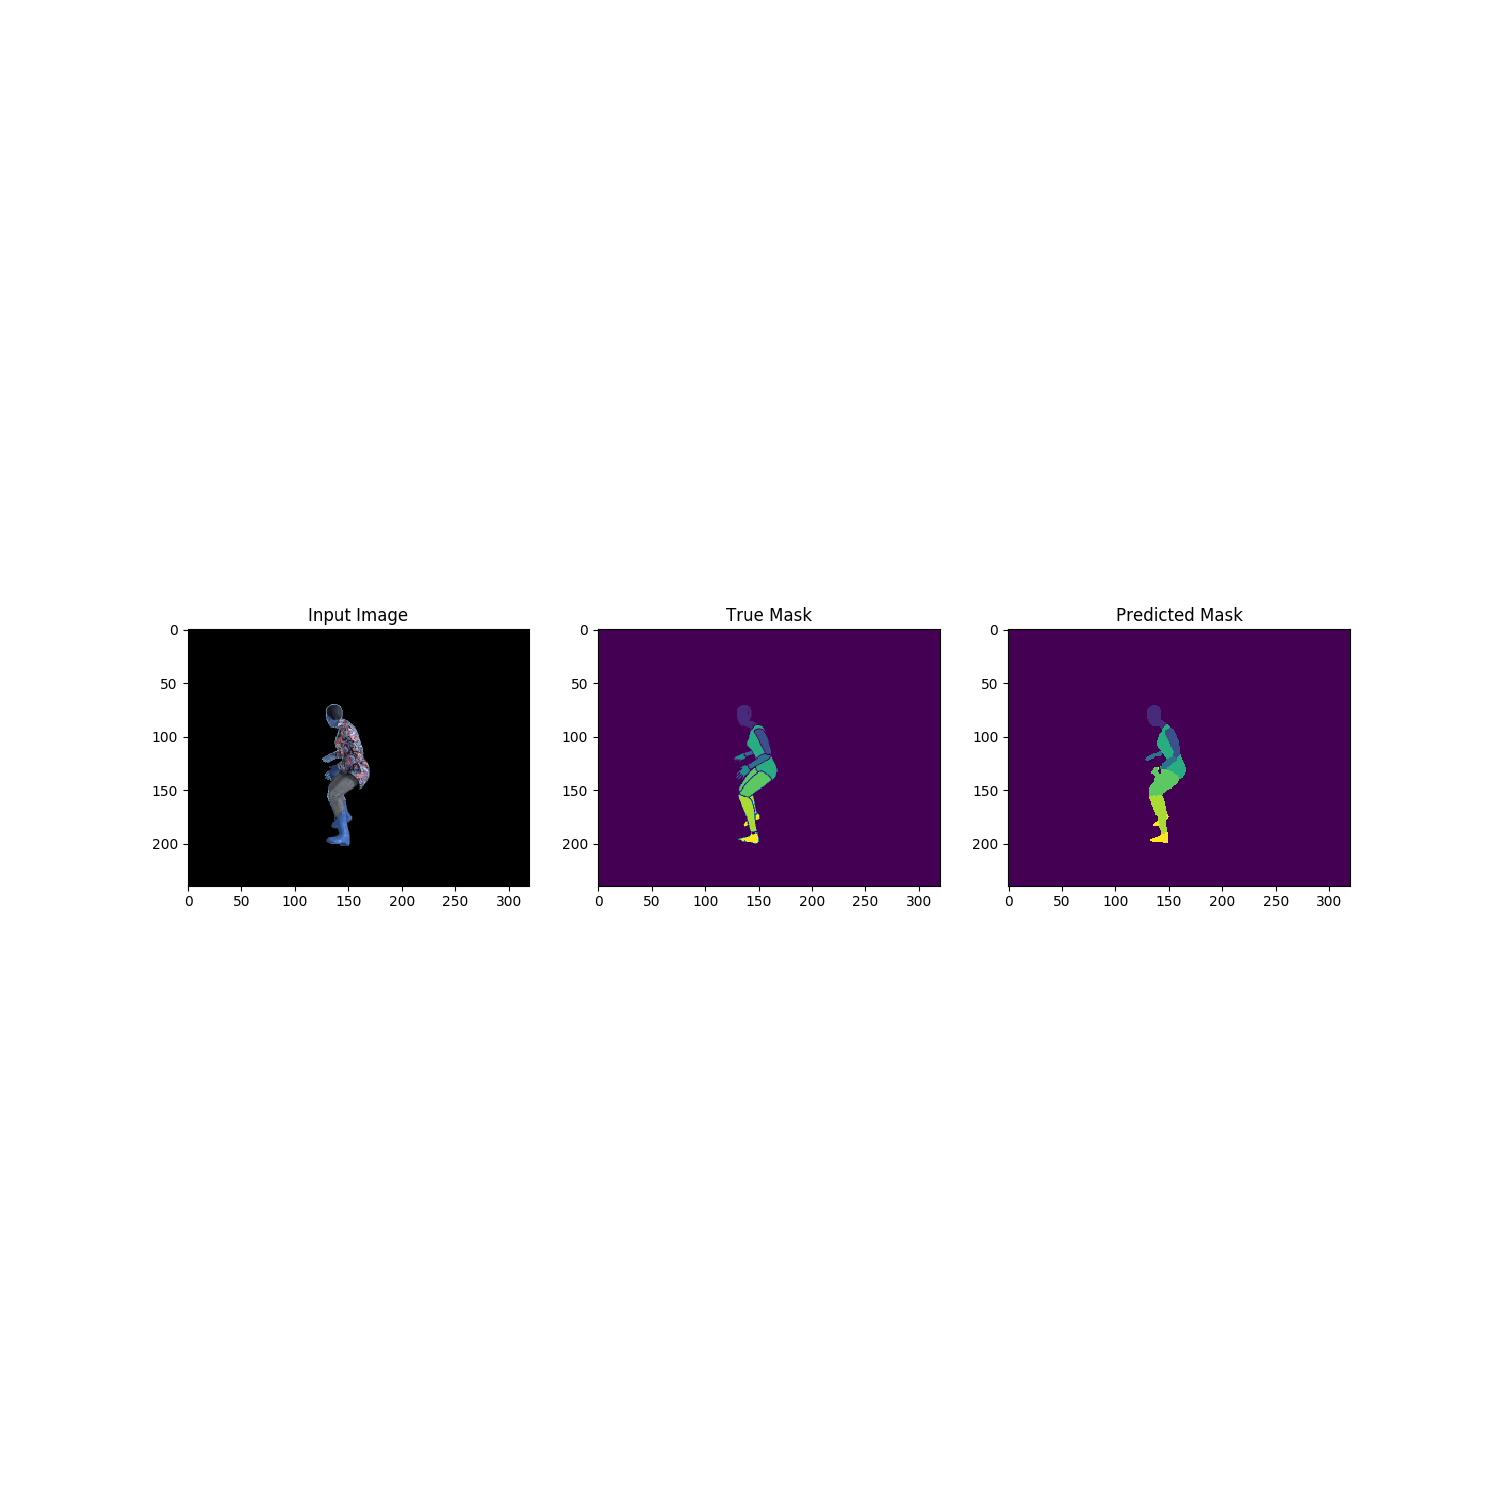
\includegraphics[width=\textwidth,height=\textheight,keepaspectratio]{img/adam_prediction_3845_train.png}
    \decoRule
    \caption[Predicted Mask]{Predicted mask after 3845. epoch with custom loss function and Adam optimizer}
    \label{fig:adam-prediction}
\end{figure}


\section{Different Net Architectures}

\subsection{Extract background }
This section will say something about training with background.
\begin{itemize}
    \item Just extract BG Module with reduced HRNet and then BP recognition
    \item BP recognition with HRNet (long training/ will this work?)
\end{itemize}

\subsection{Recognition of body parts }
\label{RBP}

\subsubsection{Stride-down, -up convolution before \gls{bl}}

\subsubsection{MobileNet extended with UNet}
\subsubsection{MobileNet extended with HRNet}

\subsubsection{Experiment with concat and add layers}

\subsubsection{Best performing network HRNet v7}

\begin{figure}[H]
    \centering
    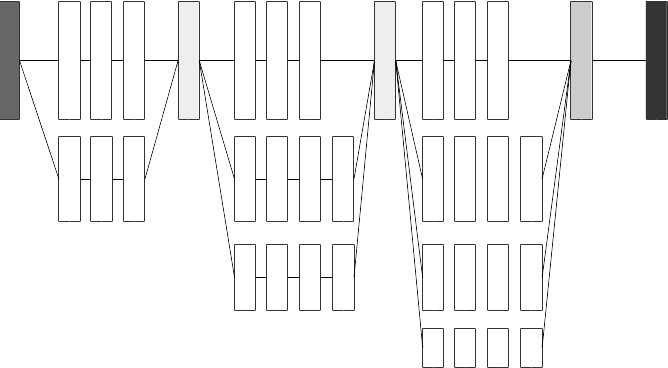
\includegraphics[width=\textwidth,height=\textheight,keepaspectratio]{img/network_v7_hrnet.png}
    \decoRule
    \caption[HRNet v7]{HRNet v7.}
    \label{fig:hrnet-v7}
\end{figure}


%-----------------------------------
%	SUBSECTION 1
%-----------------------------------


\section{Comparison of Optimizer Algorithms}

\begin{itemize}
    \item Adam
    \item Nadam
    \item SGD
    \subitem constant learning rate
    \subitem Constant decreasing learning rate
    \subitem Constant decreasing learning rate with reset of learning rate on plateau
    \subitem Increasing decreasing learning rate on plateau
\end{itemize}

\paragraph{Comparison of Adam, Nadam and SGD}
\begin{figure}[H]
    \centering
    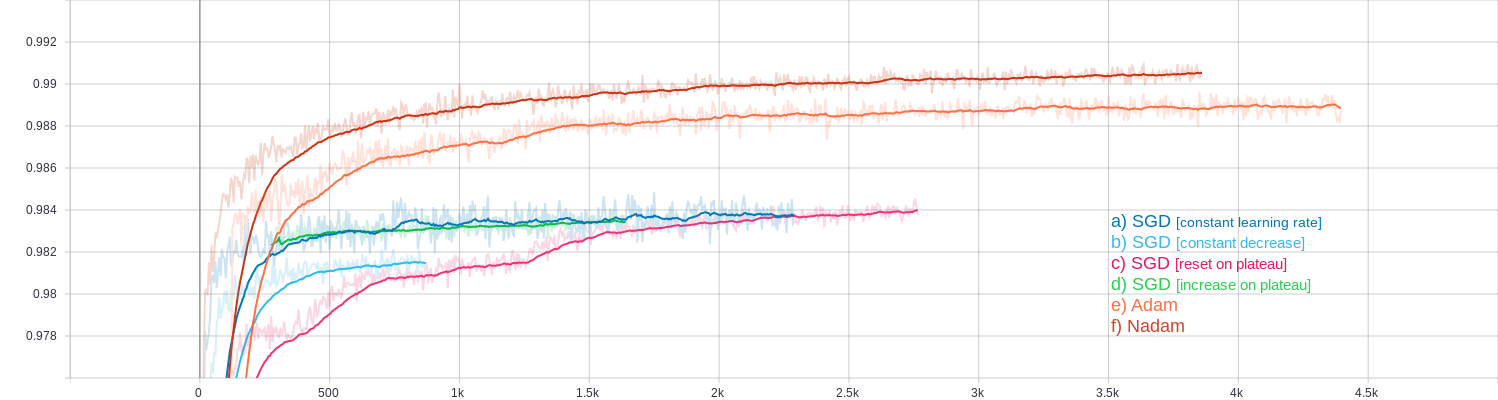
\includegraphics[width=\textwidth,height=\textheight,keepaspectratio]{img/accuracy_all.png}
    \decoRule
    \caption[Accuracy]{Accuracy}
    \label{fig:accuracy}
\end{figure}
\begin{figure}[H]
    \centering
    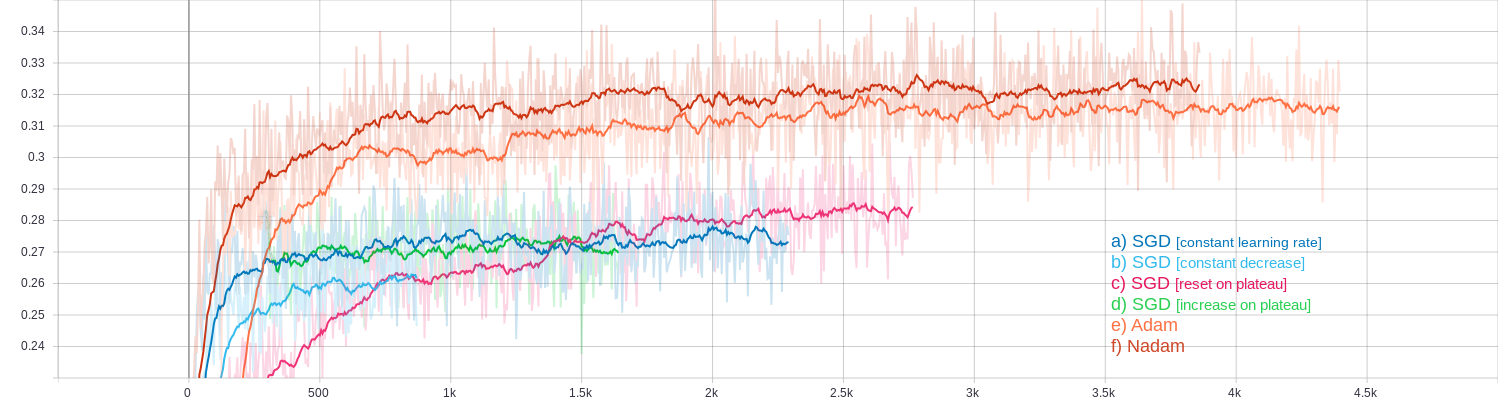
\includegraphics[width=\textwidth,height=\textheight,keepaspectratio]{img/accuracy_body_part_all.png}
    \decoRule
    \caption[Correct BPR]{Correct body part pixel relation}
    \label{fig:acc-bp}
\end{figure}
\begin{figure}[H]
    \centering
    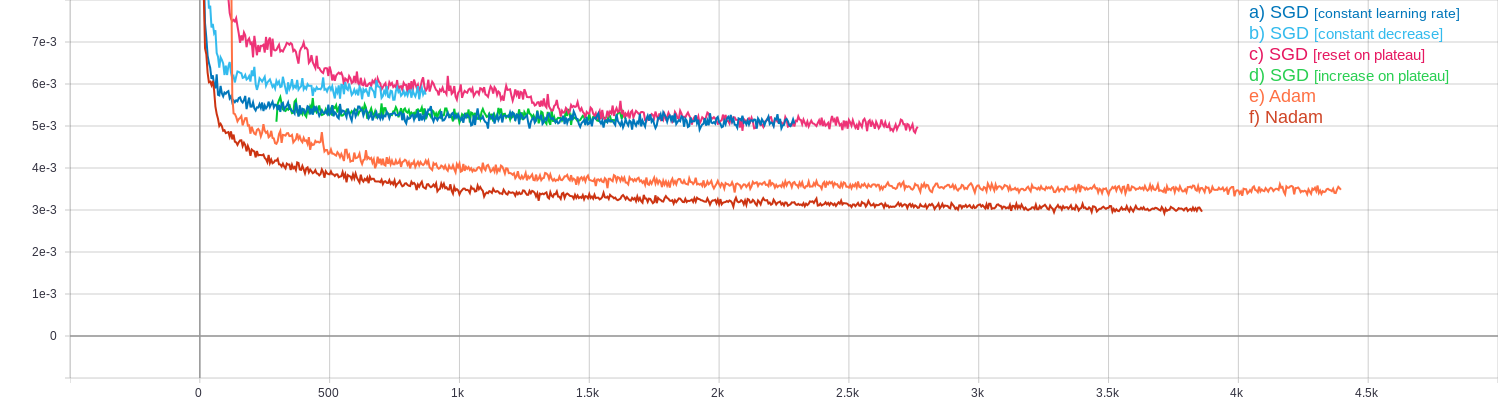
\includegraphics[width=\textwidth,height=\textheight,keepaspectratio]{img/loss_all.png}
    \decoRule
    \caption[loss]{Loss}
    \label{fig:loss}
\end{figure}

\paragraph{Experiments with SGD}
\begin{figure}[H]
    \centering
    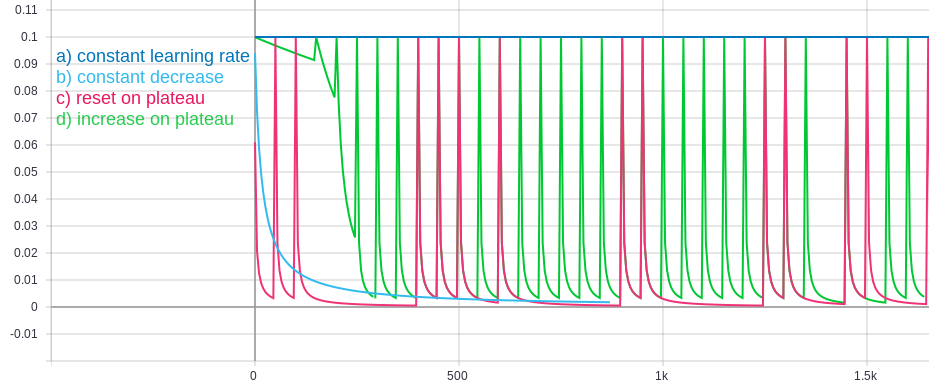
\includegraphics[width=\textwidth,height=\textheight,keepaspectratio]{img/learning_rate2.png}
    \decoRule
    \caption[Learning Rate SGD]{Learning Rate SGD.}
    \label{fig:sgd-learning-rate}
\end{figure}

\begin{figure}[H]
    \centering
    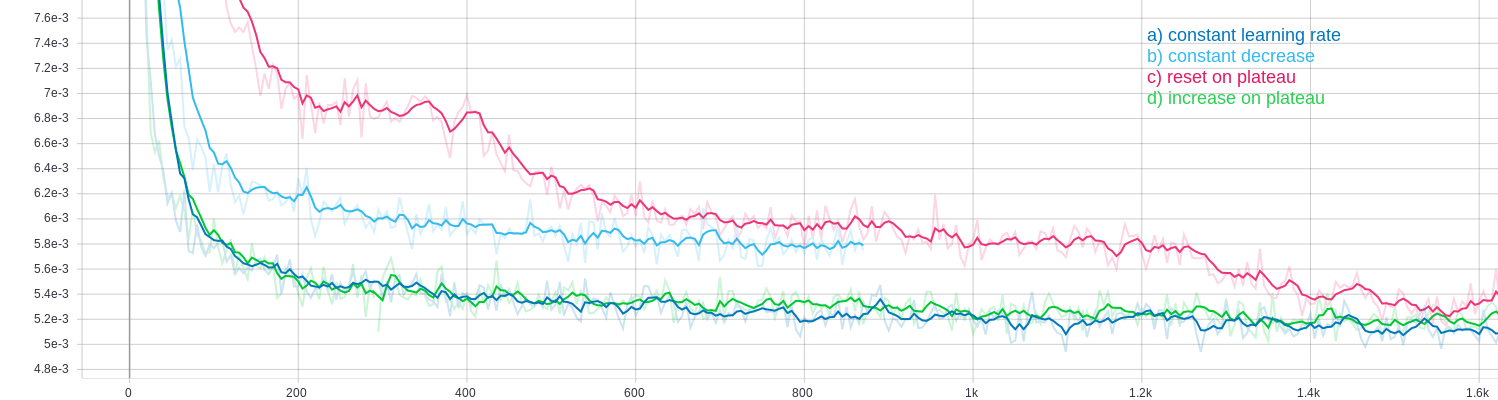
\includegraphics[width=\textwidth,height=\textheight,keepaspectratio]{img/loss_sgd.png}
    \decoRule
    \caption[Loss SGD]{Loss SGD.}
    \label{fig:sgd-loss}
\end{figure}

\begin{figure}[H]
    \centering
    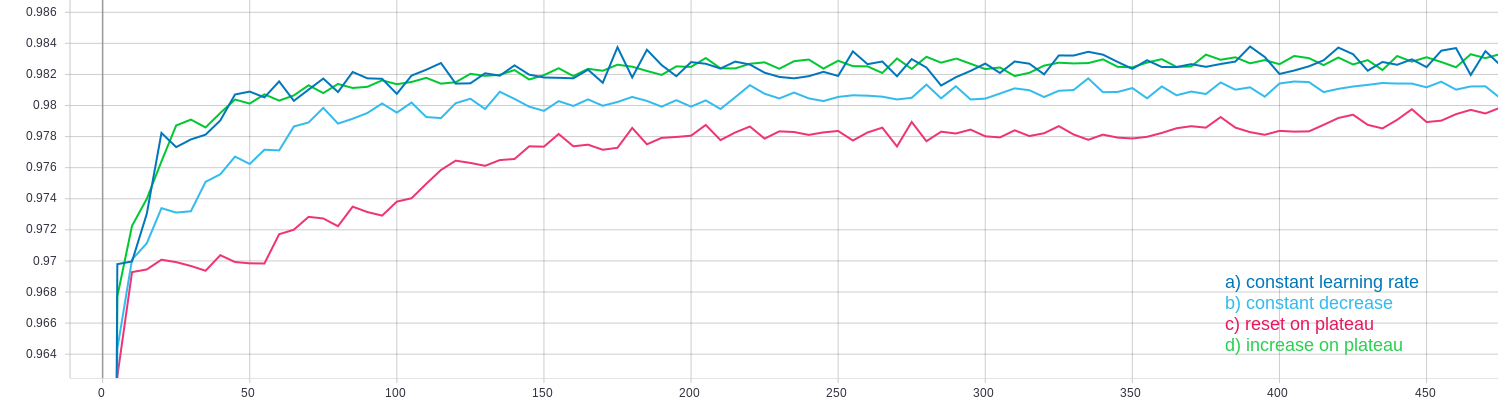
\includegraphics[width=\textwidth,height=\textheight,keepaspectratio]{img/accuracy_sgd.png}
    \decoRule
    \caption[Accuracy SGD]{Accuracy SGD.}
    \label{fig:sgd-accuracy}
\end{figure}
%-----------------------------------
%	SUBSECTION 2
%-----------------------------------

\subsection{Subsection 2}
Morbi rutrum odio eget arcu adipiscing sodales. Aenean et purus a est pulvinar pellentesque. Cras in elit neque, quis
varius elit. Phasellus fringilla, nibh eu tempus venenatis, dolor elit posuere quam, quis adipiscing urna leo nec
orci. Sed nec nulla auctor odio aliquet consequat. Ut nec nulla in ante ullamcorper aliquam at sed dolor. Phasellus
fermentum magna in augue gravida cursus. Cras sed pretium lorem. Pellentesque eget ornare odio. Proin accumsan, massa
viverra cursus pharetra, ipsum nisi lobortis velit, a malesuada dolor lorem eu neque.

%----------------------------------------------------------------------------------------
%	SECTION 2
%----------------------------------------------------------------------------------------


\section{Performance of loss functions}
All performance measures are conducted on the Nadam optimizer with the HRNet for body part recognition from
Recognition of body parts~\ref{RBP}

\subsubsection{Sparse Categorical Cross Entropy}

\subsubsection{Mean Squared Error}

\subsubsection{Our custom loss function CILoss}
This loss function confronts the problem of class imbalance, which especially occurs in body part recognition.
The background pixels appear most often, and the different body part classes occur by far less often and event they
differentiate a lot in their relative occurrence.

We try to confront this problem with a weighed map, which takes the body parts as a graph and calculates
the distances from each body part $b_x$ to all other body parts $b_n$, and stores this data inside a table.

Additionally this weight map is evened out with a multiplier to reduce the distances and facilitate
the learning process for the network.

$$\theta=y_t(x)-y_p(x)$$
$$\delta=\theta*\mu[argmax(y_t)] $$
$$L=\sum_{i=0}^{n}\theta_i+\delta_i$$


\begin{figure}[H]
    \centering
    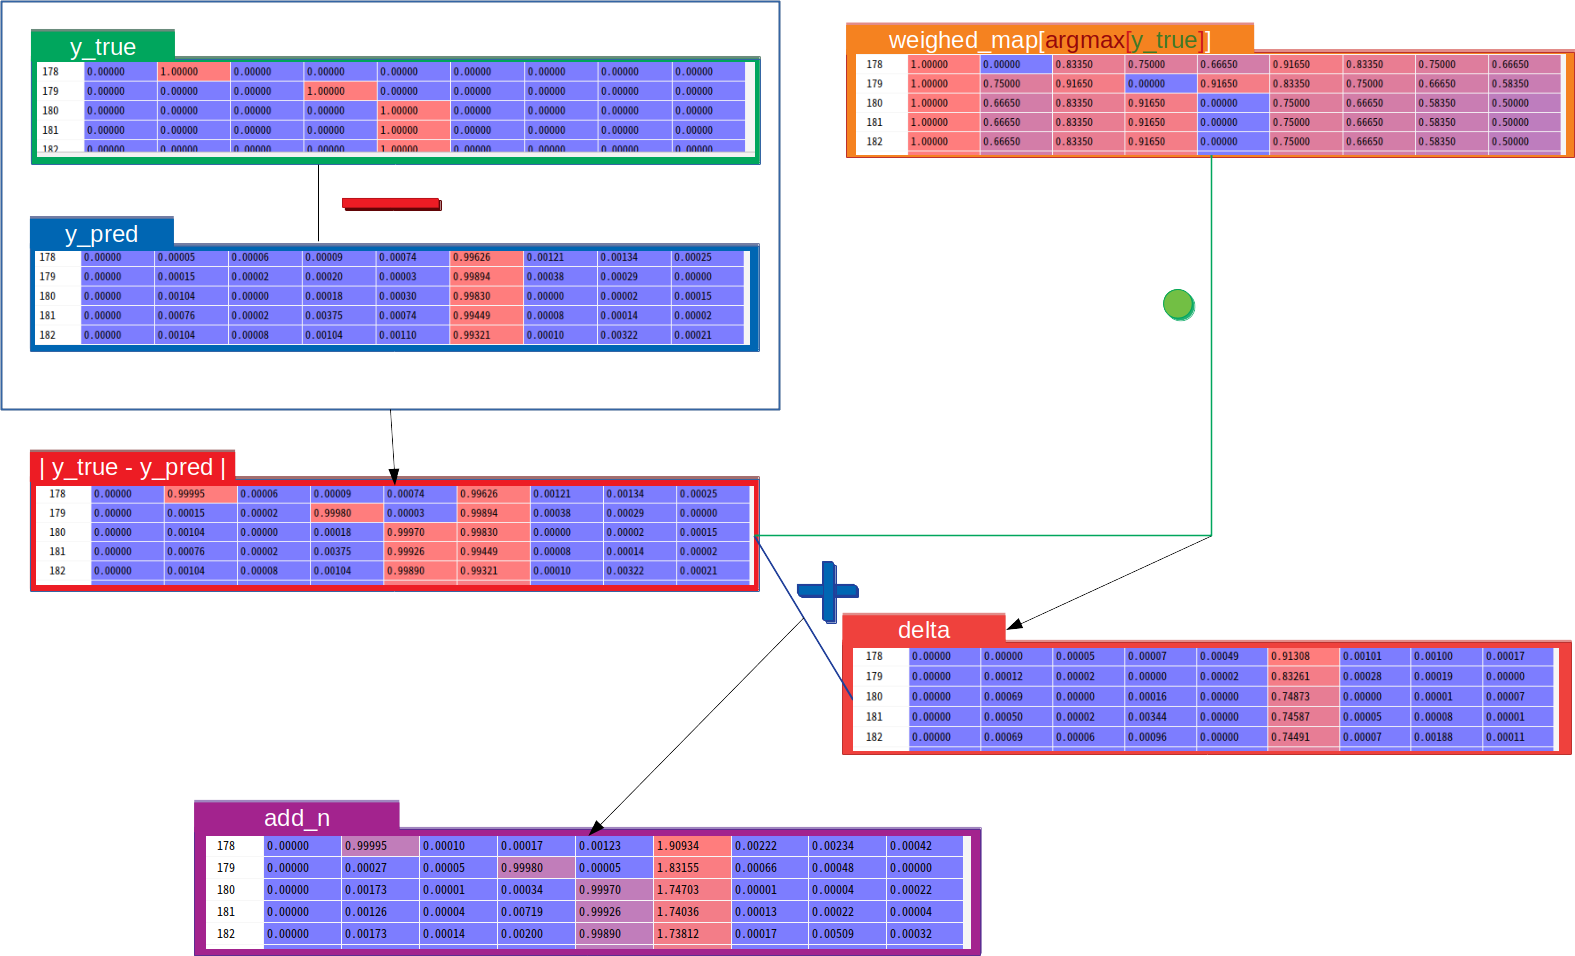
\includegraphics[width=\textwidth,height=\textheight,keepaspectratio]{img/loss_calculation.png}
    \decoRule
    \caption[CILoss]{Visualization of custom loss calculation}
    \label{fig:ciloss-calc}
\end{figure}


\section{Main Section 2}

Sed ullamcorper quam eu nisl interdum at interdum enim egestas. Aliquam placerat justo sed lectus lobortis ut porta
nisl porttitor. Vestibulum mi dolor, lacinia molestie gravida at, tempus vitae ligula. Donec eget quam sapien, in
viverra eros. Donec pellentesque justo a massa fringilla non vestibulum metus vestibulum. Vestibulum in orci quis
felis tempor lacinia. Vivamus ornare ultrices facilisis. Ut hendrerit volutpat vulputate. Morbi condimentum venenatis
augue, id porta ipsum vulputate in. Curabitur luctus tempus justo. Vestibulum risus lectus, adipiscing nec
condimentum quis, condimentum nec nisl. Aliquam dictum sagittis velit sed iaculis. Morbi tristique augue sit amet
nulla pulvinar id facilisis ligula mollis. Nam elit libero, tincidunt ut aliquam at, molestie in quam. Aenean rhoncus
vehicula hendrerit.